%
% teil3.tex -- Beispiel-File für Teil 3
%
% (c) 2020 Prof Dr Andreas Müller, Hochschule Rapperswil
%
\section{Der Munkres-Algorithmus (Ungarische Methode)
\label{munkres:section:teil3}}
\rhead{Der Munkres-Algorithmus (Ungarische Methode)}

Mit der ungarischen Methode können also Optimierungsprobleme gelöst
werden, die bei gewichteten Zuordnungen in bipartiten Graphen entstehen.
Mit ihr kann die eindeutige Zuordnung von Objekten aus zwei Gruppen so
optimiert werden, dass die Gesamtkosten minimiert werden bzw.~der
Gesamtgewinn maximiert werden kann. 

\subsection{Geschichte
\label{munkres:subsection:malorum}}
Die Ungarische Methode wurde 1955 von Harold Kuhn entwickelt und veröffentlicht.
Der Name ``Ungarische Methode'' ergab sich, weil der Algorithmus
weitestgehend auf den früheren Arbeiten zweier ungarischer Mathematiker
basierte: Dénes Kőnig und Jenő Egerváry.
James Munkres überprüfte den Algorithmus im Jahr 1957 und stellte fest,
dass der Algorithmus (stark) polynomiell ist.
Seitdem ist der Algorithmus auch als Kuhn-Munkres oder
Munkres-Zuordnungsalgorithmus bekannt.
Die Zeitkomplexität des ursprünglichen Algorithmus war $O(n^4)$,
später wurde zudem festgestellt, dass er modifiziert werden kann,
um eine  $O(n^3)$-Laufzeit zu erreichen.

\subsection{Besondere Leistung der Ungarischen Methode
\label{munkres:subsection:malorum}}
Die Ungarische Methode ist ein kombinatorischer Optimierungsalgorithmus, der das Zuordnungsproblem
in polynomieller Zeit löst.
Der Begriff polynomielle Laufzeit bedeutet, dass die Laufzeit des Programms
wie $n^2$, $n^3$, $n^4$, etc.~wächst und vernünftig skaliert. $n$ ist hierbei die "Grösse" des Problems.

\subsection{Beispiel eines händischen Verfahrens
\label{munkres:subsection:malorum}}

Die ungarische Methode kann in einem einfachen händischen Beispiel
erläutert werden. Es gibt eine Ausgangsmatrix. Diese Matrix wird in mehreren Schritten immer
weiter reduziert. Anschließend erfolgen mehrere Zuordnungen. Hierbei ist zu beachten, dass
jede Zeile und jede Spalte immer genau eine eindeutige Zuordnung ergibt.
Die optimale Lösung ist erreicht, wenn genau $n$ Zuordnungen gefunden
sind.

\begin{figure}
\centering
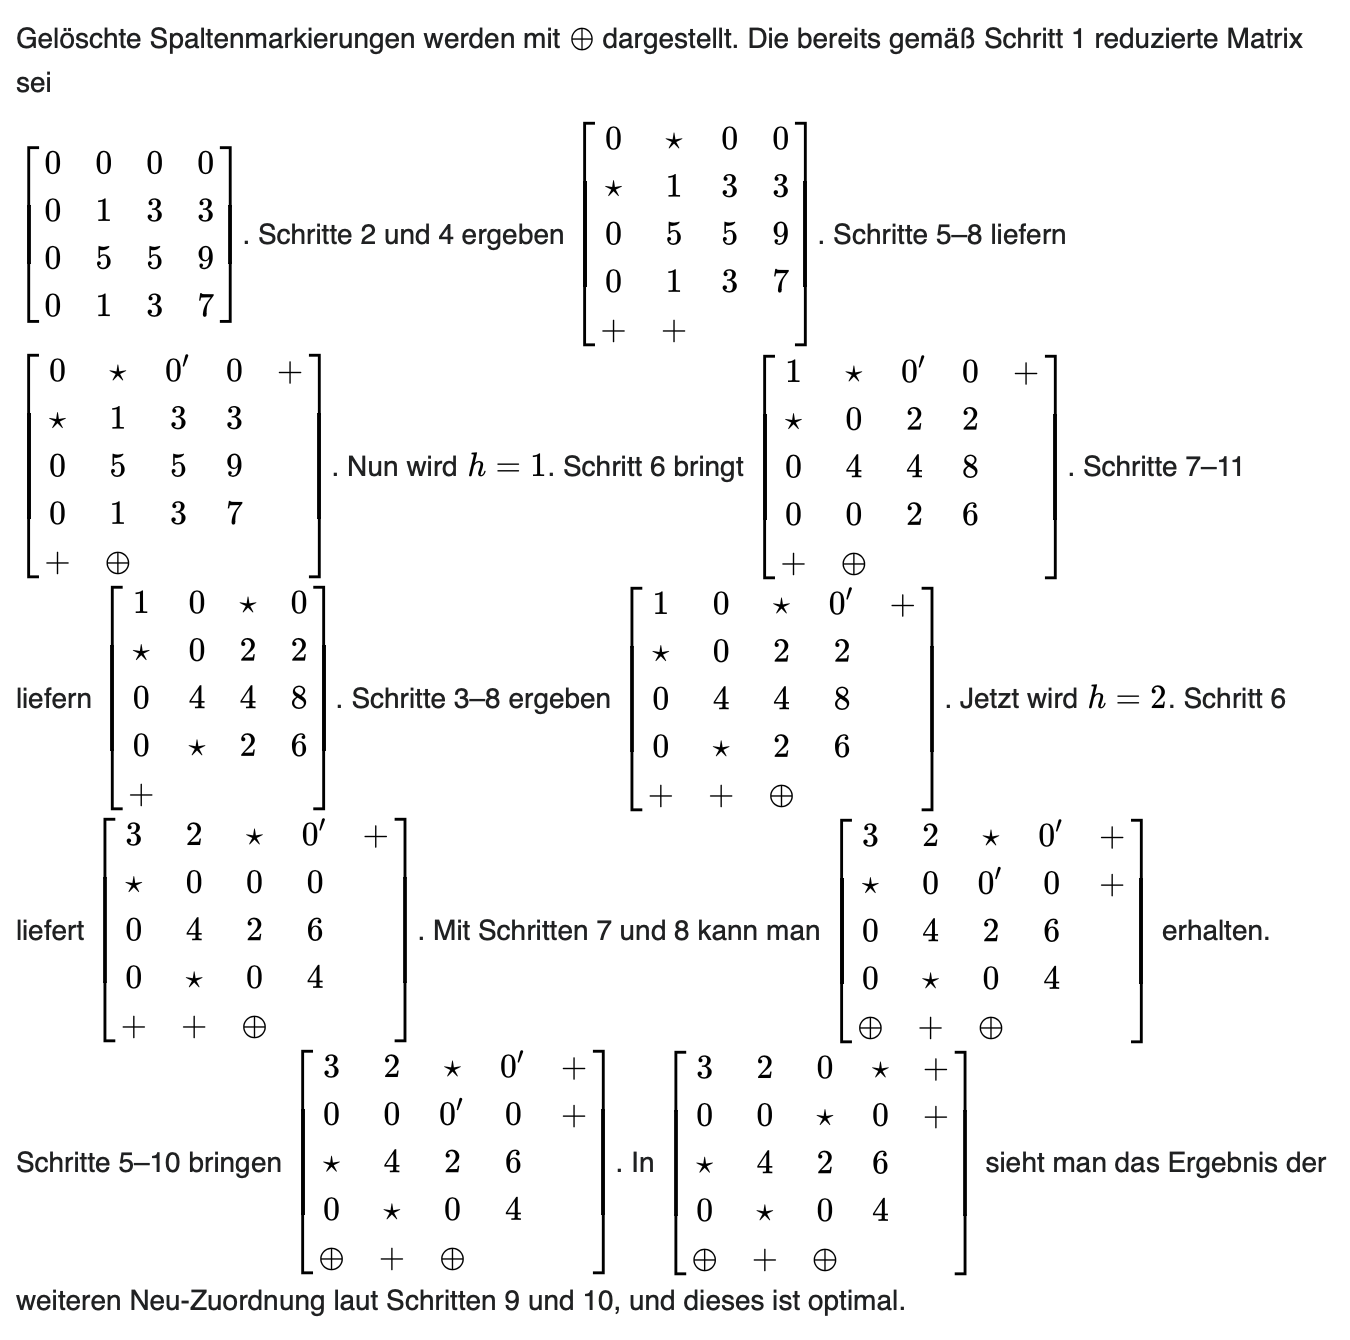
\includegraphics[width=14cm]{papers/munkres/figures/beispiel_munkres}
\caption{Händisches Beispiel des Munkres Algorithmus.}
\label{munkres:Vr2}
\end{figure}
